\documentclass[a4paper,12pt,normaltoc,capchap]{abnt}
\usepackage{abnt-UEPG}
\usepackage[top=3cm,bottom=2cm,left=3cm,right=2cm]{geometry}
\usepackage[utf8]{inputenc}
\usepackage[brazil]{babel}
\usepackage[T1]{fontenc}
%\usepackage{hyperref}
\usepackage{amssymb}
\usepackage{ae}
\usepackage{amsmath}
\usepackage{paralist}
\usepackage{graphicx}
\usepackage{subfigure}
\usepackage{setspace}
\usepackage{fancyhdr}
\usepackage{lscape}
\usepackage{longtable}
\usepackage{fancyvrb}
\usepackage{gantt}
\usepackage[alf,recuo=0cm,abnt-etal-text=it,bibjustif, abnt-emphasize = bf]{abntcite}
\usepackage{listings}
\renewcommand{\lstlistingname}{Código} % definição visual dos códigos fonte
\usepackage{inconsolata}
\usepackage[T1]{fontenc}
\usepackage{color}
\usepackage{lipsum}% just to generate text


% % % % % % % % %
%\usepackage[explicit]{titlesec}
%\usepackage{xcolor}
%\usepackage{lipsum}% just to generate text

%\colorlet{myrulecolor}{black}
%\definecolor{myrulecolor}{RGB}{150,20,0}% define the color for the rules

%\titleformat{\chapter}[display]
%  {\normalfont\scshape\Huge}
%  {\hspace*{-70pt}\thechapter.~#1}
%  {-15pt}
%  %{\hspace*{-110pt}{\color{myrulecolor}\rule{\dimexpr\textwidth+80pt\relax}{3pt}}\Huge}
%\titleformat{name=\chapter,numberless}[display]
 % {\normalfont\scshape\Huge}
 % {\hspace*{-70pt}#1}
 % {-15pt}
 % %{\hspace*{-110pt}{\color{myrulecolor}\rule{\dimexpr\textwidth+80pt\relax}{3pt}}\Huge}
%\titlespacing*{\chapter}{0pt}{0pt}{30pt}

%\titleformat{\subsection}{\normalsize\bfseries\itshape}{\textnormal{\roman{subsection}.}}{1em}{}
%\titleformat{\section}{\normalsize\bfseries\itshape}{\textnormal{\roman{subsection}.}}{1em}{}
% % % % % % % % %

\lstset{language=Java, basicstyle=\footnotesize, numbers=left, frame=tb, breaklines=true, basicstyle=\footnotesize}
\definecolor{pblue}{rgb}{0.13,0.13,1}
\definecolor{pgreen}{rgb}{0,0.5,0}
\definecolor{pred}{rgb}{0.9,0,0}
\definecolor{pgrey}{rgb}{0.46,0.45,0.48}


\newcommand{\ew}[1]		  {\emph{#1}}		% palavras em ingles 
\newcommand{\ns}[1]   	     	  {\mbox{#1}}	         	% comando para não separar palavras
\newcommand{\sigla}[1] 		  {\ns{#1}}			% comando para siglas
\newcommand{\italico}[1] 		  {\textit{#1}}		% itálico
\newcommand{\negrito}[1]  		  {\textbf{#1}}		% negrito
\newcommand{\subl}[1]	   	  {\underline{#1}}		% sublinhado
\newcommand{\X}{\textbullet}			 		% bolinha
\newcommand{\Y}{$\circ$}			 		% não preenchida


\hyphenation{pro-ces-sa-men-to}
\hyphenation{a-pre-sen-ta-da}
\hyphenation{pro-gra-ma}



\autor{UNIVERSIDADE ESTADUAL DE PONTA GROSSA \\
PRÓ-REITORIA DE PESQUISA E PÓS-GRADUAÇÃO\\
PROGRAMA DE PÓS-GRADUAÇÃO EM COMPUTAÇÃO APLICADA\\
CRISTIAN COSMOSKI RANGEL DE ABREU}

\titulo{TÉCNICAS DE COMPUTAÇÃO PARALELA PARA MELHORAR O TEMPO DA MINERAÇÃO DE DADOS:\\Uma análise de Tipos de Coberturas Florestais}

%\orientador{Profº Dr. Luciano José Senger}

%\coorientador{Profº Dr. }

\comentario{Proposta de pesquisa apresentada como um dos requisitos para obtenção do título de Mestre em Computação Aplicada na Universidade Estadual de Ponta Grossa, Área de concentração: Computação para Tecnologias Agrícolas. \\ \\Orientador: Prof. Dr. Luciano José Senger}

%\instituicao{UNIVERSIDADE ESTADUAL DE PONTA GROSSA}

\local{Ponta Grossa}

\data{2016}

%------------------------------------------------------------------------------
% Início do documento
%------------------------------------------------------------------------------

\begin{document}

\capa

\folhaderosto


%\begin{resumo}

{\noindent

O objetivo deste trabalho é investigar a utilização da computação paralela para reduzir o tempo de resposta da mineração de dados na agricultura. Para esse fim, uma ferramenta, chamada de \textit{Fast Weka} foi definida e implementada. Essa ferramenta permite executar algoritmos de mineração de dados e explorar o paralelismo em computadores multi-núcleos com o uso de \textit{threads} e em grades computacionais empregando redes \textit{peer-to-peer}. A exploração do paralelismo ocorre por meio do paralelismo de dados inerente  ao processo de validação cruzada (\textit{folds}). A ferramenta foi avaliada por meio de experimentos de mineração de dados utilizando algoritmos de redes neurais artificiais aplicados em um conjunto de dados de tipos de coberturas florestais. A computação multi-\textit{thread} e a computação em redes \textit{peer-to-peer} permitem reduzir o tempo de resposta das atividades de mineração de dados. Os melhores resultados são obtidos quando empregados um número múltiplo de \textit{threads} ou pares em relação ao número de \textit{folds} da validação cruzada. Observou-se uma eficiência de 87\% quando utilizadas 4 \textit{threads} para 24 \textit{folds} e 86\% de eficiência também com 24 \textit{folds} utilizando redes \textit{peer-to-peer} com 11 pares. \\

}
{\noindent \textbf{Palavras-chave:} Computação Paralela, Mineração de Dados, \textit{Peer-to-Peer}, Tipos de Coberturas Florestais}

\end{resumo}


%\begin{abstract}

{\noindent

The objective of this study is investigate the use of parallel computing to reduce the response time of data mining in agriculture. For this purpose, a tool, called Fast Weka been defined and implemented. This tool allows running data mining algorithms and explore parallelism in multi-core computers with the use of threads and in computational grids employing peer-to-peer networks. The exploration of parallelism occurs through the data parallelism inherent to the process of cross-validation (folds). The tool was evaluated through experiments using artificial neural networks data mining algorithms applied to a data set of forest cover types. The multi-thread computing and computing on peer-to-peer networks allow to reduce the response time of data mining activities. The best results are achieved when employed a multiple number of threads or pairs in the number of folds of cross validation. It was observed an efficiency of 87\% when used 4 threads to 24 folds and 86\% efficiency also in peer-to-peer networks using 24 folds with 11 pairs.\\

}

{\noindent \textbf{Keywords:} Parallel Computing, Data Mining, Peer-to-Peer, Forest Cover Types}
\end{abstract}


\listadefiguras

\listadetabelas
\sumario

\thispagestyle{empty}
\pagenumbering{arabic}
\setcounter{page}{4}
\chapter*{Identificação}

\begin{enumerate}

\item Aluna(o): 

\item Orientação: 

\item Coorientação: 

\item Curso: Mestrado em Computação Aplicada

\item Data de Ingresso: Janeiro/2016

\item Linha: Computação, Automação e Gestão de Dados em Agricultura.

\item Aluna(o) Regular

\end{enumerate}

\chapter{Introdução}



\section{Contextualizacao do Problema}
\lipsum[1]

\section{Justificativa}
\lipsum[1]
\section{Objetivo}
O objetivo principal deste trabalho é investigar a utilização da computação paralela afim de melhorar o tempo de resposta das atividades de mineração de dados agrícolas, avaliando e comparando os resultados obtidos nas diferentes abordagens. 
\subsection{Objetivos Específicos}

\section{Resultados Esperados}
\chapter{Revisão da Literatura}
\citeonline{Moh06} desenvolveram um trabalho utilizando MD no qual o objetivo foi desenvolver modelos para classificação de doenças do arroz egípcio. Um dos algoritmos de aprendizagem utilizado foi a RNA. A RNA foi construída e treinada utilizando uma configuração de 52 entradas, 33 neurônios na camada oculta, 5 saídas, taxa de aprendizagem de 0.3, momento de 0.2 e 500 iterações. O modelo obtido para a previsão de doenças de arroz atingiu um índice de acerto de 96,4\% para o conjunto de dados de teste. Este resultado demonstra a grande eficiência da aplicação de RNAs.

\citeonline{Bla99} realizaram a comparação entre RNA e analise discriminante para criação de classificadores para tipos de coberturas florestais a partir de variáveis cartográficas. O RNA construída utilizou as configurações de 54 entradas, 120 neurônios na camada oculta, 7 classes de tipos de coberturas florestais, com uma taxa de aprendizagem de 0.05, taxa de momento de 0.5 e 1000 interações. Para obter estas configurações para a RNA foram realizados 56 analises diferentes demandando de cerca de 56 horas para cada analise. Após a comparação das técnicas, as RNAs obtiveram uma maior precisão, chegando a 70,58\%.

\citeonline{Ala05} observou que quando o processo de aprendizado de um modelo por meio de algoritmos de aprendizagem é iniciado, este com um grande conjunto de dados, ou com um alto número de repetições, demanda de um alto custo computacional e tempo de execução. Por meio destas observações, Guimarães desenvolveu um aplicativo para distribuir o processamento da construção de seu modelo, por meio do qual o processamento poderia ser realizado por vários computadores, utilizando o algoritmo de aprendizagem Algoritmos Genéticos (AG). Este aplicativo obteve bons resultados conseguindo reduzir seu tempo de execução estimado para construção do modelo de 1450 horas para 84 horas.

\citeonline{Sou11} aplicaram uma ferramenta de MD em paralelo para construção de um modelo de classificação utilizando RNA para produção de soja, afim de observar a relação existente entre os atributos químicos do solo e a produção. Utilizando apenas um computador eles reduziram o tempo de processamento de 280 para 80 segundos. Esses resultados demostraram que a utilização de técnicas de computação paralela podem melhorar significativamente o tempo de resposta das atividades de mineração.
\lstset{language=Java,
  showspaces=false,
  showtabs=false,
  breaklines=true,
  showstringspaces=false,
  breakatwhitespace=true,
  commentstyle=\color{pgreen},
  keywordstyle=\color{pblue},
  stringstyle=\color{pred},
  basicstyle=\ttfamily,
  moredelim=[il][\textcolor{pgrey}]{$$},
  moredelim=[is][\textcolor{pgrey}]{\%\%}{\%\%}
}
\clearpage

\begin{lstlisting}[caption= Exemplo de Código em Java, label=src:java]
/**
 * This is a doc comment.
 */
package com.ociweb.jnb.lombok;

import java.util.Date;
import lombok.Data;
import lombok.EqualsAndHashCode;
import lombok.NonNull;

$$@Data
$$@EqualsAndHashCode(exclude={"address","city","state","zip"})
public class Person {
    enum Gender { Male, Female }

    // another comment

    %%@NonNull%% private String firstName;
    %%@NonNull%% private String lastName;
    %%@NonNull%% private final Gender gender;
    %%@NonNull%% private final Date dateOfBirth;

    private String ssn;
    private String address;
    private String city;
    private String state;
    private String zip;
}
\end{lstlisting}

\chapter{Materiais e Métodos}

\section{Procedimentos Experimentais}
A partir da classe com menor representatividade na base de dados, classe 4 - Algodão Americano/Salgueiro com 2.747 observações, sendo todos os dados selecionados, foram extraídas das outras seis classes de tipos de cobertura florestal 2.747 observações, selecionadas aleatoriamente com o auxilio do software R, totalizando o conjunto de teste com 19.229 observações, conforme a tabela \ref{tb:dados}.

\begin{table}[htbp]
\caption{Observações Selecionadas}
\label{tb:dados}
\centering
\setlength{\tabcolsep}{5pt}
\begin{tabular}{cccccc}
\hline
Tipo de Cobertura  &Total de  &Observações  &Porcentagem por \\
Florestal &Observações &Selecionadas &Tipo de Cobertura \\
\hline
Classe 1 &211.840 &2747 &1,29\% \\
Classe 2 &283.301 &2747 &0,97\% \\
Classe 3 &35.754  &2747 &7,68\% \\
Classe 4 &2.747   &2747 &100\% \\
Classe 5 &9.493   &2747 &28,94\% \\
Classe 6 &17.367  &2747 &15,82\% \\
Classe 7 &20.510  &2747 &13,39\% \\
\hline
\textbf{Total} &\textbf{581.012} &\textbf{19.229} &\textbf{3,31\%} \\
\hline
\end{tabular}
\\
\singlespacing
\text{\footnotesize Fonte: O autor}
\end{table}


\begin{figure}[htb]
\centering
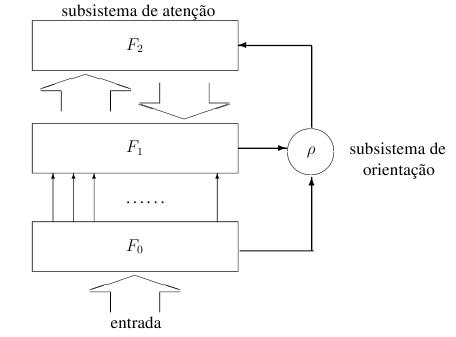
\includegraphics[scale=.5]{art}
\caption{Arquitetura da rede neural ART}\label{fig:art}
\end{figure}
\section{Análise dos Dados}


\section{Cronograma}
Visando atingir os objetivos propostos apresenta-se um cronograma
de atividades a ser realizado no âmbito do Departamento de
Automação e Sistemas (DAS/UFSC). Estas atividades e o cronograma
estão ilustrados nas tabelas \ref{tb:atividades} e
\ref{fig:cronograma}, respectivamente.

%%%% INICIO ATIVIDADES PREVISTAS %%%%%%%%%%%%%%%%%

\begin{table}[!htb]
  \centering
  \caption{Atividades Previstas}\label{tb:atividades}
  \begin{tabular}{cp{12cm}}
    \hline \hline &\\[-0.4cm]
    {\bf Atividades} & \multicolumn{1}{c}{\bf Descrição} \\
    \hline
    &\\[-0.4cm]
    \textbf{A} & Revisão bibliográfica. \\[0.2cm]
    \textbf{B} &  Estudo de novas representações.\\[0.2cm]
    \textbf{C} &  Aplicação dos algoritmos.\\[0.2cm]
    \textbf{D} &  Desenvolvimento da interface. \\[0.2cm]
    \textbf{E} &  Validação dos resultados.\\[0.2cm]
    \textbf{F} &  Elaboração da monográfia.\\[0.2cm]
    \textbf{G} &  Defesa.\\[0.2cm]
    \hline \hline
  \end{tabular}
\end{table}

%\begin{preview}
%\centering

\begin{figure}

  \begin{gantt}{10}{12}
    \begin{ganttitle}
    \numtitle{1}{1}{12}{1}
    \end{ganttitle}
    \ganttbar{Revisão da literatura}{0}{2}
    \ganttbarcon{refinamento método}{2}{5}
    \ganttbarcon{}{8}{2}
    \ganttmilestone[color=cyan]{Milestone with color!}{4}
    \ganttbar{another task}{2}{2}
    \ganttbar[color=cyan]{another coloured task}{4}{4}
    \ganttbar{another task}{4}{2}
    \ganttcon{4}{5}{4}{7}
    \ganttmilestonecon{A connected Milestone}{7}
    \ganttbarcon{another consecutive task}{8}{2}
  \end{gantt}
%\end{preview}
\caption{Cronograma de Atividades}\label{fig:cronograma}
\end{figure}
\section{Recursos}
Descrever os recursos necessários para o desenvolvimento da pesquisa.
\subsection{Recursos Humanos}
\subsection{Recursos Físicos}



\chapter{Considerações Finais}
Fique atento aos principais problemas que podem ocorrer ao elaborar o projeto de dissertação, os quais podem comprometer o mesmo: 
\begin{itemize}
\item	O objetivo é muito amplo, geral ou vago;
\item	O projeto ignora conhecimentos anteriores já acumulados sobre o objeto de investigação;
\item	A revisão de literatura não apresenta o estado da arte efetivo ou ela é inadequada e não se articula com o objeto de investigação;
\item	O objeto de investigação não é interdisciplinar se enquadra nos campos de atuação da linha de pesquisa na qual o aluno se insere; 
\item	O objeto de investigação não se enquadra nos campos de atuação da linha de pesquisa na qual o aluno se insere; 
\item	O objeto de investigação é pouco relevante;
\item	A descrição da metodologia ou  inadequada ao objeto de investigação;  
\item	O impacto científico/tecnológico da investigação proposta não é enfatizado ou é pouco relevante; 
\item	Cronograma é irrealista ou não contempla as atividades necessárias.
\end{itemize}  



\bibliographystyle{abnt-alf}
\bibliography{base}

%\include{Apendice}

\end{document}
